\chapter{Extensibility of GP}
\label{ch3:extensibility}

Recalling from Figure~\ref{f:optflow}, traditional gradient-based design optimization tools implement
convergence loops that assume structure within a given design problem.
The 'bag of constraints' form of the GP means that constraints can be
added to the problem without
having to restructure the optimization formulation. This property,
coupled with the object-oriented modeling framework of GPkit, allows
\gls{GP} compatible models to be continuously extensible.
In this section, I will demonstrate common methods used to extend the capability
and improve the fidelity of \gls{GP}- and \gls{SP} compatible models.

\section{Improving fidelity: Adding a simple engine model to the SimPleAC}
\label{s:engine}

The SimPleAC currently has an engine that weighs nothing and magically supplies
unlimited power. This is obviously unphysical, and requires refinement.

\subsection{Creating an engine submodel}

Before even thinking about modeling, we would like to leverage the object-oriented
GPkit models to put the variables describing the engine into a submodel (currently only
BSFC). We do this by creating a new class called \textbf{Engine} and creating a \textit{setup}
method that returns the constraints within it.

\begin{python}
    class Engine(Model):
        def setup(self):
            # Dimensional constants
            BSFC = Variable("BSFC", 400, "g/(kw*hr)", "brake specific fuel consumption")
            constraints = []
            return constraints
\end{python}

We allow the SimPleAC model to contain the variables and constraints of the engine
as follows:

\begin{python}
    class SimPleAC(Model):
        def setup(self):
            self.engine = Engine()
            self.components = [self.engine]
            ...
            return constraints, self.components
\end{python}

This restructuring of the model yields the exact same overall \gls{GP} formulation
as the unstructured problem, but gives us the flexibility to develop submodels
collaboratively and in a disciplined manner.

If we think of an engine as an input-output system, we can determine how it
would interact with the SimPleAC system, and create appropriately bounded
sets of variables.
At the most basic level, the engine provides shaft power, consumes fuel,
and has weight. The model is missing both the shaft power and weight description
of the engine. If we abstract away the propeller (the relation between shaft
power and thrust power) through a propeller efficiency,
we can perhaps relate maximum power to weight.

\subsection{Data-based modeling: engine power vs. weight}
\label{s:datafit}

We can imagine that, for a specific kind of engine, there is a relation between the
maximum shaft power available and the mass of the engine, somewhat related to the
cube-square law, which describes the relation between the surface area and volume
of objects. And let's assume that our knowledge of the internal workings of engines
is limited, but we have some knowledge of the technology available in the market
and have data to support it. Using GPfit, we will try to fit the data to find
\gls{GP} compatible relations between engine weight and maximum power. This section
will try to highlight the best practices when making data-based models.

To be able to fit the engine power vs. weight data, we take several important steps.
\begin{itemize}
    \item \textbf{Comb the data.} Since we are essentially projecting
    data with potentially high standard deviation onto a single line,
    it is important to fit the ranges of data we care about.
    \item \textbf{Normalize the data.} Normalizing the data
    by some known quantity is preferable, fits should not be dependent on the
    units that are used while performing it. This also helps the fit integrate
    seamlessly into GPkit, since dimensional fits would require units manipulation
    to avoid errors. The data can be normalized by any
    reference quantities (in this case using the maximum power and weight values
    from the data set).
    \item \textbf{Choose the type of fit.} In~\cite{gpfitpaper}, \textit{softmax-affine}
    (SMA) and \textit{implicit softmax-affine} (ISMA)
    functions are proposed and implemented as convex approximations
    to data. Depending on the behavior of the data, one or the other
    may be appropriate. For engineering relations that are expected to be smooth, SMA
    functions are often good approximations. However, if kinks are expected in the
    functions, ISMA functions can locally adjust the softness of the fit to
    reduce the error of the fit.
    \item \textbf{Choose the number of posynomial terms in the fit.} The number of
    terms will likely depend on the root-mean square (RMS) error of the fit, and
    the kind of pressure on the variable. RMS error can be reduced by including
    more posynomial terms, but only if the variable of interest has downward
    pressure on it from the objective function (since it is on the greater side
    of the inequality).
\end{itemize}

After having performed these intermediate steps on the engine data,
the relation we obtain for the one-term approximation is as follows:
\begin{equation}
    \left(\frac{W_{eng}}{W_{eng,max}}\right)^{0.100} = 0.988 \left(\frac{P_{shaft}}{P_{shaft,max}}\right)^{0.117}
\end{equation}

Note that the root mean square error of this fit is 0.414, which primarily has to do with
the level of variation in the data. Since engine weight will have downward pressure
on it from the objective, we can easily use a two-term posynomial approximation to
improve its error.

\begin{equation}
    \left(\frac{W_{eng}}{W_{eng,max}}\right)^{0.801} \geq 0.0330 \left(\frac{P_{shaft}}{P_{shaft,max}}\right)^{0.167}
    +1.59 \left(\frac{P_{shaft}}{P_{shaft,max}}\right)^{1.36}
\end{equation}

This relation has an r.m.s. error of 0.346, which is a significant improvement.
Both fits are shown with the data in Figure~\ref{f:enginefit}.

\begin{figure}
    \centering
    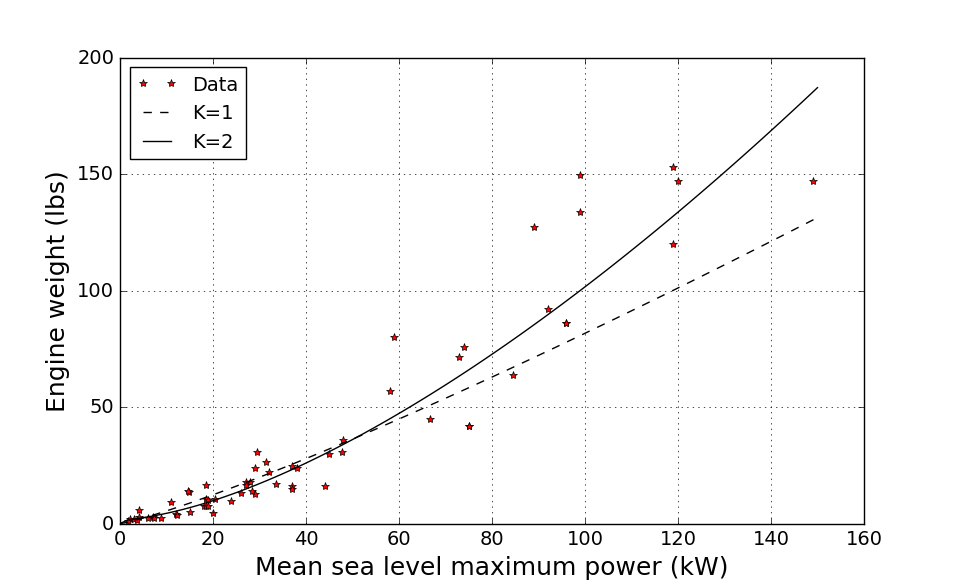
\includegraphics[width=0.6\textwidth]{enginePvsW.png}
    \caption{Engine MSL power versus weight fits for $K=1,2$ posynomial terms with underlying data.}
    \label{f:enginefit}
\end{figure}

It turns out that with a SMA approximation, more terms do not improve the r.m.s.
error of the fit on the given data. As such, we will proceed with the 2-term posynomial fit.

\subsubsection{Other constraints in engine model}

I constrain the cruise shaft power to be 20\% of the maximum shaft power of the engine,
to account for engine surge power demands. This rather arbitrary constraint is removed
later when the full mission model is integrated.

\begin{equation}
    P_{shaft} \leq \frac{1}{5} P_{shaft,max}
\end{equation}

\subsection{Converting all subsystems into submodels}
\label{s:submodels}

Within this framework, we can modularize also add a separate wing and fuselage module to
SimPleAC as well, with very little additional work. This creates the variable and constraint
hierarchy as presented in Figure~\ref{forest:submodels}, which define all of the constraints
required for SimPleAC to fly one flight segment.

\begin{figure}[!h]
    \centering\small\sffamily
    \begin{forest}
        sn edges
        [\textbf{Aircraft}
        [\textbf{Wing}]
        [\textbf{Fuselage}]
        [\textbf{Engine}]
        ]
    \end{forest}
    \caption{Variable and constraint hierarchy of the single mission segment SimPleAC model}
    \label{forest:submodels}
\end{figure}

Tree structures such as in Figure~\ref{forest:submodels} are informative, since
it provides an intuitive representation of the way constraints and variables
are passed between GPkit models. The way the \gls{SP} is solved at the end has no
hierarchy, but as we will see in Section~\ref{s:mission} a hierarchical representation
will facilitate the vectorization of constraints required for mission design.

%TODO: develop on the idea of variable and constraint hierarchy

\section{Mission design and performance modeling form}
\label{s:mission}

The SimPleAC that I have defined so far works well to demonstrate the
capabilities of \gls{SP} in helping explore tradeoffs in engineering design.
However, often in the design process, we will want to test the performance of a
design in different conditions, and/or during different phases of a mission.
This requires the vectorization of
constraints that relate to the performance of the design. What we'd like to do
is to have a single aircraft optimize both its static sizing variables (having
to do with the airframe), and its flight performance simultaneously. This requires a major
augmentation of the model tree defined in Figure~\ref{forest:submodels}, into a
uni-directional graph as shown in Figure~\ref{f:missiongraph}.

\begin{figure}[!h]
    \centering\small\sffamily
    \begin{forest}
        sn edges,
        l sep+=1em,
        for children={
        l sep+=1em,
        }
        [\textit{\textbf{Mission}},name=mission
        [\textit{\textbf{\shortstack{Aircraft\\Perf.}}},name=aircraftP2
        [\textit{\shortstack{Wing\\Perf.}},name=wingP2]
        [\textit{\shortstack{Engine\\Perf.}},name=engineP2
        [\textit{Atmosphere},name=atmos2]]]
        [,name=phantom
        [\textbf{Aircraft},name=aircraft
        [\textbf{Wing},name=wing]
        [\textbf{Fuselage},name=fuse]
        [\textbf{Engine},name=engine]
        ]]
        [\textit{\textbf{\shortstack{Aircraft\\Perf.}}},name=aircraftP1
        [\textit{\shortstack{Wing\\Perf.}},name=wingP1]
        [\textit{\shortstack{Engine\\Perf.}},name=engineP1
        [\textit{Atmosphere},name=atmos1]]
        ]
        ]
        \draw[->] (atmos1) -- (wingP1);
        \draw[->] (atmos1) -- (aircraftP1);
        \draw[->] (atmos2) -- (wingP2);
        \draw[->] (atmos2) -- (aircraftP2);
        \draw[->] (aircraft) -- (aircraftP1);
        \draw[->] (aircraft) -- (aircraftP2);
        \draw[->] (wing) -- (wingP1);
        \draw[->] (engine) -- (engineP1);
        \draw[->] (wing) -- (wingP2);
        \draw[->] (engine) -- (engineP2);
        \node[draw,rectangle,fit={(aircraftP2) (atmos2) (engineP2) (wingP2)}] {};
        \node[draw,rectangle,fit={(aircraftP1) (atmos1) (engineP1) (wingP1)}] {};
    \end{forest}
    \caption{Variable and constraint hierarchy of the presented aircraft model, for two flight
    segments. Models that include sizing variables are
    bolded while models that include performance variables are italicized.
    There are models that contain both kinds of variables.}
    \label{f:missiongraph}
\end{figure}

The performance models are enclosed in a rectangle, and they are
vectorized by the number of flight segments, $N_{segments}$. Each
one of the performance models contain variables that change between flight segments.
Note that I have created a performance model for all subcomponents other than the
fuselage. This is because the only performance variable of the fuselage is its drag
coefficient, which is assumed to not change between flight segments, making it static. I
have also added a \textbf{\textit{Mission}} model, which links flight segments together,
and an \textit{Atmosphere} model, which describes the conditions in which the aircraft
operates.

The static aircraft model, and the atmospheric state are passed as an argument to multiple
performance models within this framework. To transform our previously static model to
the performance-static model hierarchy we have identified,
we have to determine which variables
belong in which level of the tree. Table~\ref{t:missionvars} details the full
decomposition of the model into its submodels in the format defined
by Figure~\ref{f:missiongraph}. This is as simple as identifying which variables
we do not expect to change during flight segments, and which ones we do.

\begin{center}
    \captionof{table}{Variables of SimPleAC in performance modeling, detailed in the
    variable and constraint hierarchy.}
    {\footnotesize
\begin{longtable}{lcl}
\toprule
Free Variables & Units & Description \\ \midrule
\multicolumn{3}{l}{\textbf{Mission}} \\
$W_{f_{m}}$ & $~\mathrm{N}$ & Total mission fuel \\
$t_m$ & $~\mathrm{hr}$ & Total mission time \\
$R_s$ & $~\mathrm{km}$ & Range flown in segment \\
$W_{avg}$ & $~\mathrm{N}$ & Segment average weight \\
$W_{end}$ & $~\mathrm{N}$ & Weight at the end of flight segment \\
$W_{f_s}$ & $~\mathrm{N}$ & Segment fuel burn \\
$W_{start}$ & $~\mathrm{N}$ & Weight at the beginning of flight segment \\
$\frac{\Delta h}{dt}$ & $~\mathrm{\tfrac{m}{hr}}$ & Climb rate \\
$h$ & $~\mathrm{m}$ & Flight altitude \\
$t_s$ & $~\mathrm{hr}$ & Time spent in flight segment \\
\hline
\multicolumn{3}{l}{\textbf{Mission/Atmosphere}} \\
$\mu$ & $~\mathrm{\tfrac{kg}{\left(m\cdot s\right)}}$ & dynamic viscosity \\
$\rho$ & $~\mathrm{\tfrac{kg}{m^{3}}}$ & density of air \\
$h$ & $~\mathrm{m}$ & altitude \\
\hline
\multicolumn{3}{l}{\textbf{Mission/SimPleAC}} \\
$V_f$ & $~\mathrm{m^{3}}$ & maximum fuel volume \\
$V_{f_{avail}}$ & $~\mathrm{m^{3}}$ & fuel volume available \\
$W$ & $~\mathrm{N}$ & maximum takeoff weight \\
$W_f$ & $~\mathrm{N}$ & maximum fuel weight \\
\hline
\multicolumn{3}{l}{\textbf{Mission/SimPleAC/Engine}} \\
$P_{shaft_{max}}$ & $~\mathrm{kW}$ & MSL maximum shaft power \\
$W_e$ & $~\mathrm{N}$ & engine weight \\
\hline
\multicolumn{3}{l}{\textbf{Mission/SimPleAC/Fuselage}} \\
$(CDA0)$ & $~\mathrm{m^{2}}$ & fuselage drag area \\
$C_{D_{fuse}}$ & $$ & fuselage drag coefficient \\
$V_{f_{fuse}}$ & $~\mathrm{m^{3}}$ & fuel volume in the fuselage \\
\hline
\multicolumn{3}{l}{\textbf{Mission/SimPleAC/Wing}} \\
$A$ & $$ & aspect ratio \\
$S$ & $~\mathrm{m^{2}}$ & total wing area \\
$V_{f_{wing}}$ & $~\mathrm{m^{3}}$ & fuel volume in the wing \\
$W_w$ & $~\mathrm{N}$ & wing weight \\
$W_{w_{strc}}$ & $~\mathrm{N}$ & wing structural weight \\
$W_{w_{surf}}$ & $~\mathrm{N}$ & wing skin weight \\
\hline
\multicolumn{3}{l}{\textbf{Mission/SimPleACP}} \\
$C_D$ & $$ & drag coefficient \\
$D$ & $~\mathrm{N}$ & total drag force \\
$L/D$ & $$ & lift-to-drag ratio \\
$Re$ & $$ & Reynolds number \\
$V$ & $~\mathrm{\tfrac{m}{s}}$ & cruising speed \\
\hline
\multicolumn{3}{l}{\textbf{Mission/SimPleACP/EngineP}} \\
$P_{shaft}$ & $~\mathrm{kW}$ & shaft power \\
$T$ & $~\mathrm{N}$ & propeller thrust \\
\hline
\multicolumn{3}{l}{\textbf{Mission/SimPleACP/WingP}} \\
$C_L$ & $$ & wing lift coefficient \\
$C_f$ & $$ & skin friction coefficient \\
$C_{D_{ind}}$ & $$ & wing induced drag \\
$C_{D_{wpar}}$ & $$ & wing profile drag \\
\bottomrule
\end{longtable}}

{\footnotesize
\begin{longtable}{lcl}
\toprule
Constants & Units & Description \\ \midrule
\multicolumn{3}{l}{\textbf{Mission}} \\
$Cost Index$ & $~\mathrm{\tfrac{1}{hr}}$ & hourly cost index \\
$Range$ & $~\mathrm{km}$ & aircraft range \\
$V_{min}$ & $~\mathrm{\tfrac{m}{s}}$ & takeoff speed \\
$W_p$ & $~\mathrm{N}$ & payload weight \\
\hline
\multicolumn{3}{l}{\textbf{Mission/Atmosphere}} \\
$P_{MSL}$ & $~\mathrm{Pa}$ & pressure at MSL \\
$T_{MSL}$ & $~\mathrm{K}$ & temperature at MSL \\
$\mu_{MSL}$ & $~\mathrm{\tfrac{kg}{\left(m\cdot s\right)}}$ & dynamic viscosity at MSL \\
$\nu_{MSL}$ & $~\mathrm{\tfrac{m^{2}}{s}}$ & kinematic viscosity at MSL \\
$\rho_{MSL}$ & $~\mathrm{\tfrac{kg}{m^{3}}}$ & density of air at MSL \\
$a_{MSL}$ & $~\mathrm{\tfrac{m}{s}}$ & Speed of sound at MSL \\
$h_{top}$ & $~\mathrm{m}$ & highest altitude valid \\
\hline
\multicolumn{3}{l}{\textbf{Mission/SimPleAC}} \\
$\rho_f$ & $~\mathrm{\tfrac{kg}{m^{3}}}$ & density of fuel \\
$g$ & $~\mathrm{\tfrac{m}{s^{2}}}$ & gravitational acceleration \\
\hline
\multicolumn{3}{l}{\textbf{Mission/SimPleAC/Engine}} \\
$P_{shaft_{ref}}$ & $~\mathrm{kW}$ & reference MSL maximum shaft power \\
$W_{e_{ref}}$ & $~\mathrm{N}$ & reference engine weight \\
$\eta_{prop}$ & $$ & propeller efficiency \\
\hline
\multicolumn{3}{l}{\textbf{Mission/SimPleAC/Wing}} \\
$(\frac{S}{S_{wet}})$ & $$ & wetted area ratio \\
$C_{L,max}$ & $$ & max CL with flaps down \\
$N_{ult}$ & $$ & ultimate load factor \\
$W_{w_{coeff1}}$ & $~\mathrm{\tfrac{1}{m}}$ & wing weight coefficent 1 \\
$W_{w_{coeff2}}$ & $~\mathrm{Pa}$ & wing weight coefficent 2 \\
$\tau$ & $$ & airfoil thickness to chord ratio \\
$e$ & $$ & Oswald efficiency factor \\
$k$ & $$ & form factor \\
\hline
\multicolumn{3}{l}{\textbf{Mission/SimPleACP/EngineP}} \\
$BSFC$ & $~\mathrm{\tfrac{g}{\left(hr\cdot kW\right)}}$ & thrust specific fuel consumption \\
\bottomrule
\end{longtable}}
{\footnotesize
\begin{longtable}{lcl}
\toprule
Sensitivities & Units & Description \\ \midrule
\multicolumn{3}{l}{\textbf{Mission}} \\
$Range$ & $~\mathrm{km}$ & aircraft range \\
$V_{min}$ & $~\mathrm{\tfrac{m}{s}}$ & takeoff speed \\
$Cost Index$ & $~\mathrm{\tfrac{1}{hr}}$ & hourly cost index \\
$W_p$ & $~\mathrm{N}$ & payload weight \\
\hline
\multicolumn{3}{l}{\textbf{Mission/Atmosphere}} \\
$\rho_{MSL}$ & $~\mathrm{\tfrac{kg}{m^{3}}}$ & density of air at MSL \\
$\mu_{MSL}$ & $~\mathrm{\tfrac{kg}{\left(m\cdot s\right)}}$ & dynamic viscosity at MSL \\
$h_{top}$ & $~\mathrm{m}$ & highest altitude valid \\
\hline
\multicolumn{3}{l}{\textbf{Mission/SimPleAC}} \\
$g$ & $~\mathrm{\tfrac{m}{s^{2}}}$ & gravitational acceleration \\
$\rho_f$ & $~\mathrm{\tfrac{kg}{m^{3}}}$ & density of fuel \\
\hline
\multicolumn{3}{l}{\textbf{Mission/SimPleAC/Engine}} \\
$\eta_{prop}$ & $$ & propeller efficiency \\
$P_{shaft_{ref}}$ & $~\mathrm{kW}$ & reference MSL maximum shaft power \\
$W_{e_{ref}}$ & $~\mathrm{N}$ & reference engine weight \\
\hline
\multicolumn{3}{l}{\textbf{Mission/SimPleAC/Wing}} \\
$(\frac{S}{S_{wet}})$ & $$ & wetted area ratio \\
$k$ & $$ & form factor \\
$C_{L,max}$ & $$ & max CL with flaps down \\
$e$ & $$ & Oswald efficiency factor \\
$\tau$ & $$ & airfoil thickness to chord ratio \\
$W_{w_{coeff2}}$ & $~\mathrm{Pa}$ & wing weight coefficent 2 \\
$N_{ult}$ & $$ & ultimate load factor \\
$W_{w_{coeff1}}$ & $~\mathrm{\tfrac{1}{m}}$ & wing weight coefficent 1 \\
\hline
\multicolumn{3}{l}{\textbf{Mission/SimPleACP/EngineP}} \\
$BSFC$ & $~\mathrm{\tfrac{g}{\left(hr\cdot kW\right)}}$ & thrust specific fuel consumption \\
\bottomrule
\end{longtable}}

    \label{t:missionvars}
\end{center}

Then, using the variable structure in Table~\ref{t:missionvars}, we can place the
constraints in the appropriate locations. Each constraint should be placed
in the model that contains the variable in the constraint that is highest in the level of hierarchy. For example,
we can consider the constraint for thrust power in Equation~\ref{e:thrustConstr}.

\begin{equation}
    \label{e:thrustConstr}
    T \times V \leq \eta_{prop} P_{shaft}
\end{equation}

We expect that thrust ($T$) and shaft power ($P_{shaft}$) occur
in \textit{Engine Performance}. Since our model has no model for propeller efficiency ($\eta_{prop}$), we treat it
as a static variable in \textbf{Engine}. And velocity ($V$) is a variable in \textbf{\textit{Aircraft {Performance}}}.
As a result, the constraint for thrust power would logically reside in the \textbf{\textit{Aircraft {Performance}}}
model, the highest level in the hierarchy as shown in Figure~\ref{f:thrustConstr}. Since this model is vectorized,
the constraint would be vectorized by the number of flight segments we create.

\begin{figure}[!h]
    \centering\small\sffamily
    \begin{forest}
    [\textit{\textbf{Mission}},name=mission
    [\textit{\textbf{\shortstack{Aircraft\\Perf.}}},name=aircraftP
    [\textbf{Aircraft},name=aircraft
    [\textbf{Wing},name=wing]
    [\textbf{Fuselage},name=fuse]
    [\textbf{Engine},name=engine]
    ]
    [\textit{\shortstack{Wing\\Perf.}},name=wingP]
    [\textit{\shortstack{Engine\\Perf.}},name=engineP
    [\textit{Atmosphere},name=atmos]]
    ]
    ]
        \draw[->] (atmos) -- (wingP);
        \draw[->] (atmos) -- (aircraftP);
        \draw[->] (aircraft) -- (aircraftP);
        \draw[->] (aircraft) -- (mission);
        \draw[->] (wing) -- (wingP);
        \draw[->] (engine) -- (engineP);
        \node[draw,rectangle,fit={(engineP)}] {};
        \node[draw,rectangle,fit={(aircraftP)}] {};
        \node[draw,rectangle,fit={(engine)}] {};
    \end{forest}
    \caption{The models that contain the variables in Equation~\ref{e:thrustConstr} are enclosed in rectangles.
    Constraint logically resides in \textbf{\textit{Aircraft Perf.}}.
    The vectorization of performance models has been neglected for clarity.}
    \label{f:thrustConstr}
\end{figure}

Now, we have used a framework to modularize our constraints, which makes it
amenable to vectorization and mission design.

\subsection{Linking performance models: flight segments}

Although the variables in the performance models are vectorized, they can be constrained
against each other. If each of the \textit{\textbf{Aircraft Performance}} models were operating
independently of
each other simulating different missions, then they would simply be merged in the bag of constraints
of \textbf{\textit{Mission}}. However, we know that the models are related through since the aircraft
burns fuel throughout the mission, changing its flight characteristics.

The derivation of the \gls{GP}-compatible flight segment models has been detailed in ~\cite{gassolar}
and used widely within the \gls{CEG} in aircraft design. It defines segment start, end and average weights,
as well as altitude, and all of its relevant constraints are contained in the \textbf{\textit{Mission}}
model.

I have added the monomial equality below to the formulation from~\cite{gassolar}

\begin{align}
    h_{{avg}_1} &= \frac{1}{2}\Delta h_1 \\
    h_{{avg}_i} &= \sqrt{h_{i} \times h_{i-1}}, \quad i = 2,...,N_{segments}
\end{align}

to add an average altitude variable $h_{avg}$ in Section~\ref{s:atmos}. This adds
conservatism to the density and drag (otherwise, the air density for a flight segment is calculated
at the end of the segment, at which the aircraft is at its highest altitude). I have also constrained
the cruise altitude (final altitude in every flight segment but the initial segment) to be greater than 5000m.

As with most \gls{GP} approximations, there are limitations to this model. To avoid non-positive
altitude change values ($\Delta h$), we restrict the aircraft to climb during every segment, and
don't model descents. Furthermore, we have binned the flight segments to equal range segments to
avoid the potential lower-unboundedness of the lengths of certain segments.

\subsection{Characterizing the environment: atmospheric model}
\label{s:atmos}

We have created a mission and flight segment model without having we have to have a better understanding
of the environment in which the aircraft operates. So far, we have assumed that
the aircraft flies at a constant altitude (sea level) for a single mission segment,
and is subject to the same air density and viscosity. This is a big simplification
that we can overcome through vectorization.

I have borrowed Tony Tao's atmosphere fits, which are 2-term softmax-affine fits of the atmospheric
quantities of interest ($\rho$ and $\mu$ in this thesis) with respect to altitude. The constraints
are guaranteed to be tight through signomial equalities.
The relations are valid between 0-10000m of altitude.

Similar environmental models can be made for other design problems where the environmental
variables are inextricably coupled to performance.

\subsection{Objective of the mission model}

Recalling from Section~\ref{s:altobj}, upper-unbounded performance metrics often have to
reside in the objective function to be bounded. As such, I have added mission time $t_m$ through a cost index as such:

\begin{equation}
    \mathrm{Objective} \geq W_f \frac{1}{\mathrm{N}} + \mathrm{Cost Index} \times t_m
    \label{e:missionobj}
\end{equation}

I have added $\mathrm{Cost Index}$ as a separate variable so that we can observe the sensitivity
of the variable post-optimization.

\section{Design exploration through mission design}

There are a few interesting methods that are specific to mission design that we can use to explore
potential designs using\gls{GP}s.

Leveraging the speed of convex optimization, we can perform sweeps with respect to mission input
parameters, and map out the entire design space w.r.t the objective. In this case, I have chosen to
sweep across both payload weight and range, and the variable of interest is mission fuel weight.
Note that
every point in the design space represents a fully optimized aircraft.

\begin{figure*}[t!]
    \centering
    \begin{subfigure}[t]{0.5\linewidth}
        \centering
        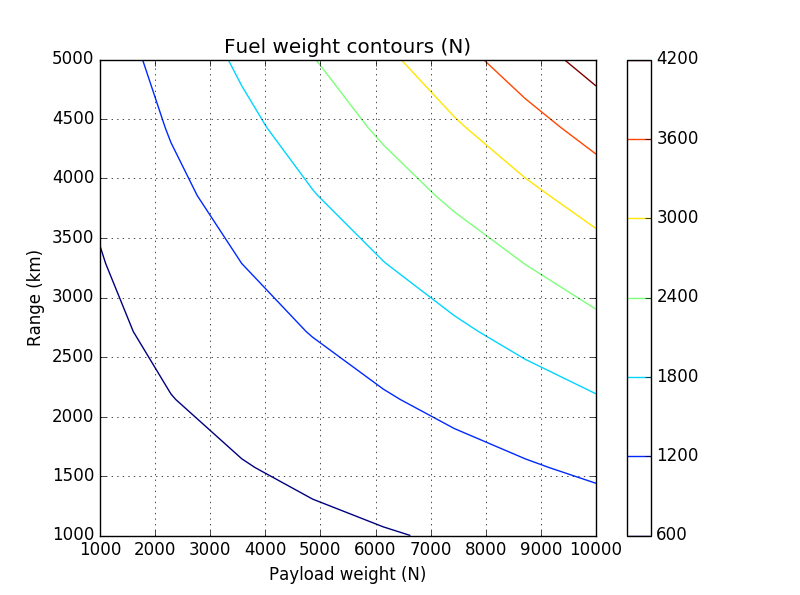
\includegraphics[width=0.9\linewidth]{W_fcontours.png}
    \end{subfigure}%
    ~
    \begin{subfigure}[t]{0.5\linewidth}
        \centering
        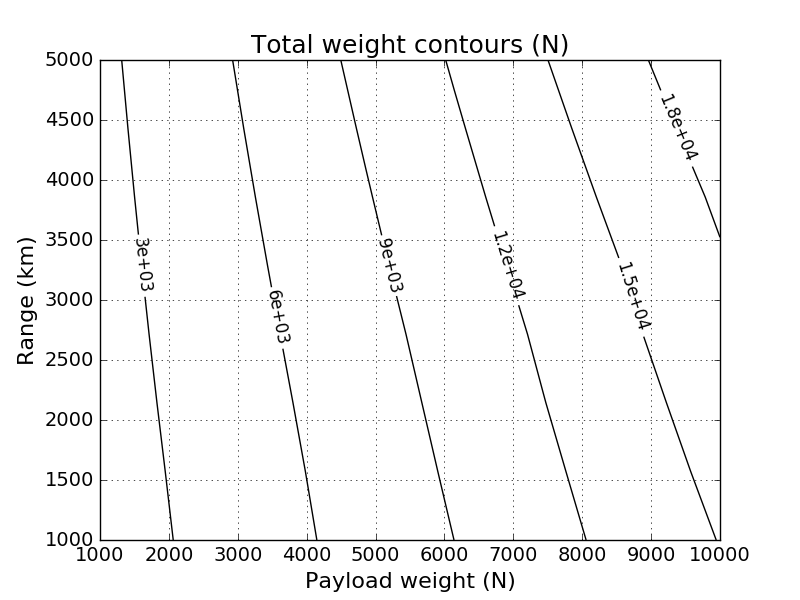
\includegraphics[width=0.9\linewidth]{Wcontours.png}
    \end{subfigure}
    \caption{The fuel and total weight Pareto frontiers with respect to range and payload inputs.}
    \label{f:pareto}
\end{figure*}

In Section~\ref{s:fuel} we had to weigh whether or not it was worth losing the mathematical
guarantees of convexity to be able to model fuel storage. Now we can use our \gls{SP} model to understand
the tradeoffs in fuel storage, and when it is beneficial to store fuel in the wing versus the fuselage.

\begin{center}
\begin{figure}
    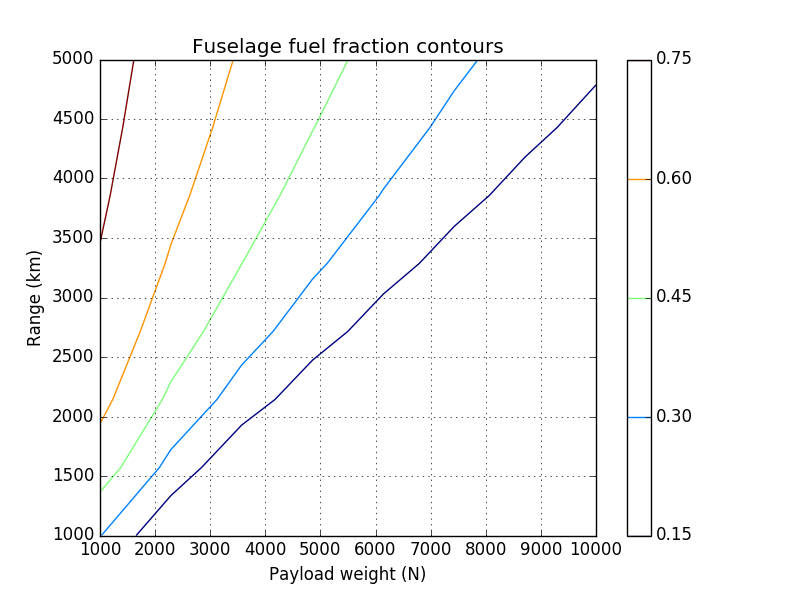
\includegraphics[width=0.45\linewidth]{FuseFuelFraccontours.png}
    \caption{}
    \label{f:fusefuelfrac}
\end{figure}
\end{center}

Figure~\ref{f:fusefuelfrac} shows how designs for different range and payload requirements
allocate fuel differently within the aircraft. As the mission range increases for a given payload weight,
more and more fuel is allocated within the fuselage as a proportion of total fuel. Since fuselage fuel
volume is directly related to increased fuselage drag, it makes sense that no fuel is put in the fuselage
until the fuel volume constraint in the wing becomes tight. And this is the behavior that is observed.

\section{Improved modeling in mission design}

There are still significant weaknesses in the model that mission design often exploits to arrive at solutions
that do not seem physical. In this specific modeling example, it shows the weaknesses of the engine model.

The first weakness is the fact that the engine can supply the same amount of power
regardless of altitude. For naturally aspirated piston engines, we would expect the maximum power available to
drop with altitude; adding such a lapse rate will improve how much we trust the engine model.
The second is the lack of an engine \BSFC model. As an aerospace engineer, I have the insight
empirically that the \BSFC of an engine deteriorates at low power outputs.  Using more
data-based modeling, we can model this relationship and improve our results.

In Sections~\ref{s:lapse} and \ref{s:BSFC}, I will aim to implement these improvements. Then in Section\ref{s:compare},
we can see how improved modeling affects the results of the model.

\subsection{Engine lapse rate model}
\label{s:lapse}

I have described how we can perform data-based modeling in Section~\ref{s:datafit}, so I will
not linger here. But much in the same way I created posynomial fits for the relationship between
engine maximum power and weight, I have created a posynomial fit for the lapse rate of the engine.
This models requires the insertion of another signomial equality into the model. Consider the
posynomial inequality expression below:

\begin{equation}
    \label{e:lapse}
    1 \geq L + \frac{P_{shaft,alt}}{P_{shaft,max}}
\end{equation}

Since the \BSFC of a normally aspirated piston engine would be expected to improve
as the $P_{shaft} \xrightarrow[]{} P_{shaft,alt}$, the maximum shaft
power at altitude has downward pressure on it from the fuel burn objective. This means that the
inequality doesn't adequately lower bound the $P_{shaft,alt}$. If we try to flip the inequality in
Constraint~\ref{e:lapse}, then $P_{shaft,alt}$ is upper-unbounded, so with our current parametrization
of the shaft power, we must use a signomial equality.

\subsection{Making use of sensitivities: engine \BSFC model}
\label{s:BSFC}

The \BSFC is one of the variables that the model is most sensitive to, and it has yet to be modeled. As
stated in Section~\ref{s:lapse}, the \BSFC of a piston engine improves as the engine puts out more power.

BSFC has downward pressure due to the objective function, and therefore must be lower-bounded. This makes
it amenable to multiple-term posynomial fits.

First, I attempted a monomial fit of the $\frac{\BSFC}{\BSFC_{min}}$ versus $\frac{P_{shaft}}{P_{shaft,alt}}$.
The result is shown in Figure~\ref{f:P_BSFC}.

\begin{center}
    \begin{figure}
        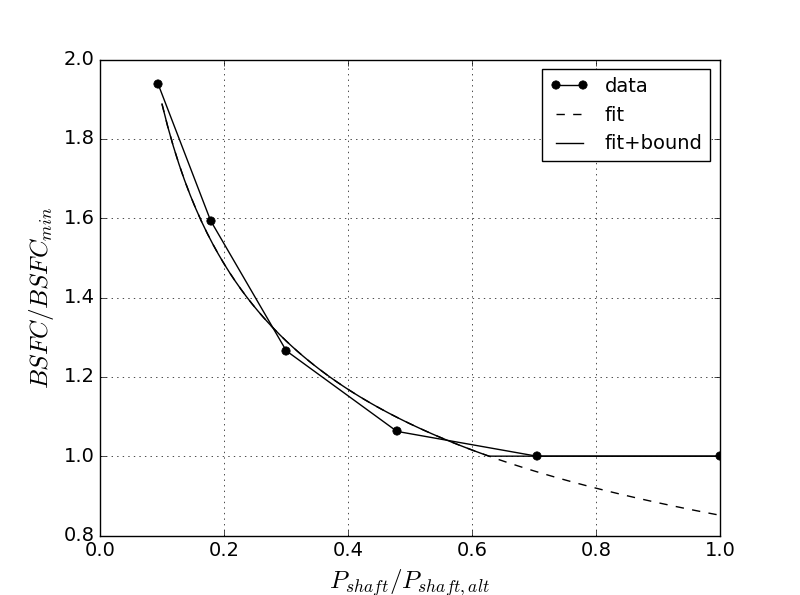
\includegraphics[width=0.5\textwidth]{P_BSFC.png}
        \caption{$\frac{\BSFC}{\BSFC_{min}}$ versus $\frac{P_{shaft}}{P_{shaft,alt}}$ data fit. Note that the fit is
        not able to capture the tail ends of the curve.}
        \label{f:P_BSFC}
    \end{figure}
\end{center}

Although the r.m.s. error of the fit is low (0.015), there is a significant deterioration in the quality of the
fit as $\frac{P_{shaft}}{P_{shaft,alt}} \xrightarrow[]{} 1$,
and increasing the number of posynomial terms in the fit does not alleviate this problem. It
turns out that fitting with respect to lapse rate using the simple relation $1 = L + \frac{P_{shaft}}{P_{shaft,alt}}$
resolves the issue. The fit with respect to lapse rate, which has been implemented in the model, is
shown in Figure~\ref{f:lapse_BSFC.png}

\begin{center}
    \begin{figure}
        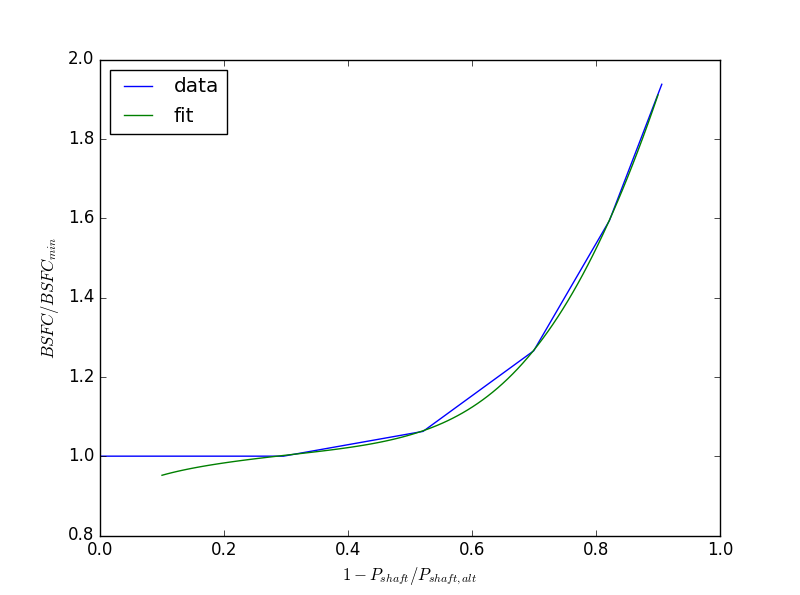
\includegraphics[width=0.5\textwidth]{lapse_BSFC.png}
        \caption{Engine lapse \% $L$ versus $\frac{P_{shaft}}{P_{shaft,alt}}$ data fit. This fit has minimal
        RMS error.}
        \label{f:lapse_BSFC}
    \end{figure}
\end{center}

The r.m.s. error of the new fit is less than $10^{-10}$, since we are able to find a 2-term posynomial that
goes through the seven data points to numerical precision.
The improvement of the fit thanks to a simple variable transformation shows that
parametrization can be important to the level of accuracy and fidelity of a model.

\subsection{Comparing models under different sets of constraints}
\label{s:compare}

Now we can compare the changes in the results, both in terms of the mission and airframe design, with respect
to the improved engine model.

%TODO: add table with the input values to initial and final missions

%TODO: add table comparing the results of the different missions

And most importantly, we should see changes in the sensitivity contours that may (or sometimes may not)
agree with our engineering intuition. This is a valuable feature of optimization coupled in design.

\subsection{Insights from mission design}

\begin{center}
\begin{figure}
    \includegraphics[width=0.45\linewidth]{h_cruisesenscontours.png}
    \caption{}
    \label{f:h_cruisesens}
\end{figure}
\end{center}

Another interesting aspect to investigate is the effect of minimum cruise altitude. In none of the designs
does minimum cruise altitude have a zero sensitivity, which indicates that the constraint is always tight.
However, we do observe that, if the



\section{Multimission design}
\label{s:multimission}

Having created a mission profile for the SimPleAC, it only takes one extra level of
hierarchy to do multimission design. Now we vectorize the mission models flown by the same aircraft.

%\begin{figure}[!h]
%    \centering\small\sffamily
%    \begin{forest}
%        sn edges
%        [\textit{\textbf{Multimission}},name=multimission
%        [\textit{\textbf{Mission}},name=mission1
%        [\textit{\textbf{\shortstack{Aircraft\\Perf.}}},name=ap1]
%        [\textit{\textbf{\shortstack{Aircraft\\Perf.}}},name=ap2]
%        ]
%        [\textbf{Aircraft},name=ac]
%        [\textit{\textbf{Mission}},name=mission2
%        [\textit{\textbf{\shortstack{Aircraft\\Perf.}}},name=ap3]
%        [\textit{\textbf{\shortstack{Aircraft\\Perf.}}},name=ap4]
%        ]
%        ]
%
%        \draw[->] (ac) -- (ap1);
%        \draw[->] (ac) -- (ap2);
%        \draw[->] (ac) -- (ap3);
%        \draw[->] (ac) -- (ap4);
%
%    \end{forest}
%    \caption{Multimission uni-directional graph.}
%    \label{f:multimission}
%\end{figure}

Now the vectorization has gone down two levels. We are able to consider $N$ flight segments, $M$


